\chapter{Introduzione}

Nel corso di Laboratorio di Fisica dei Plasmi siamo interessati a plasmi non neutri, ossia dei sistemi a molti corpi
costituiti da particelle cariche che presentano una carica netta globale. Sistemi di questo genere sono caratterizzati
dalla presenza di forti campi elettrici legati alla natura non neutra dell'insieme di particelle considerato: tali campi
possono avere grande influenza sul comportamento del plasma e sulle proprietà del regime di stabilità che si può instaurare.
I plasmi non-neutri più semplici sono quelli costituiti da singole specie cariche: a questa categoria appartengono i plasmi 
di elettroni prodotti in laboratorio.

In certe condizioni i plasmi non-neutri possono essere descritti utilizzando una trattazione macroscopica fluido-dinamica, per 
esempio  i \textit{plasmi freddi} si comportano come dei fluidi ideali bidimensionali: questo parallelismo consente di effettuare 
esperimenti per testare il comportamento di un fluido ideale. Questa non è l'unica utilità scientifica dei plasmi prodotti in 
laboratorio, poichè essi sono stati utilizzati anche per creare anti-materia, mescolando plasmi di positroni e di anti-protoni.

I plasmi non neutri costituiti da specie con cariche tutte dello stesso segno possono essere confinati con facilità maggiore 
rispetto ai plasmi neutri: i non-neutri possono essere delimitati in una specifica regione di spazio utilizzando solo campi 
elettrici e magnetici statici in una configurazione nota con il nome di \textit{trappola di Malmberg-Penning}.
\begin{figure}[H]
  \centering
  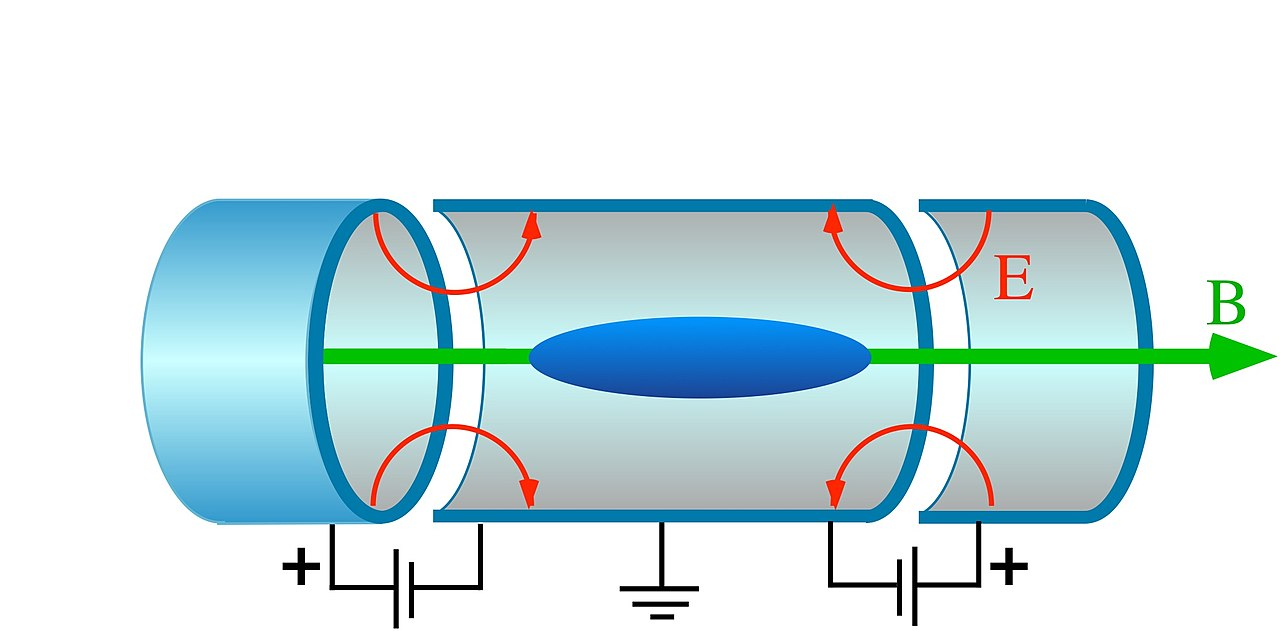
\includegraphics[width=0.75\textwidth]{Immagini/Penning_Trap.jpg}
  \caption{ Versione cilindrica della trappola di Penning: B indica il campo magnetico, mentre E è il campo
  elettrico usato per tenere le particelle nel centro.}
  \label{figure: PenningTrap}
\end{figure}

\section{Struttura della dispensa}

La dispensa si articola nei seguenti capitoli:
\begin{enumerate}
    \item In questo capitolo abbiamo introdotto la tipologia di fenomeni fisici che ci proponiamo di trattare
    e studiare sperimentalmente.
    \item Nel Capitolo 2 vengono introdotte alcune tecniche teoriche che consentono di studiare le caratteristiche principali
    dei plasmi non-neutri, ponendo particolare enfasi sugli equilibri che interessano le esperienze di laboratorio.
    \item Nel Capitolo 3 viene introdotta l'instabilità di Diocotron, che sarà argomento di almeno un'esperienza in laboratorio 
    ed è un'instabilità onnipresente nell'evoluzione di un plasma a bassa densità.
  \end{enumerate}
